\section{Simulation} \label{sec: Simulation}
Describes the result of the behavioral simulation based on the synthesized hardware description language.
The most important module to simulate is the state machine because it includes the logic applied out of the state diagram. 
One problem by simulating out of the top level are the clock divider which would need way more simulation time then 1000 ns therefore it is good practice to simulate each module once and proof its function by writing individual test bench files for each module.
Figure \ref{fig: Simulation_state_machine} shows the simulated state machine with the state gum. By using radix for the char01 to char 12 signals an easy readable simulated result can be achieved.
For an extended report more simulations would be added and explained in more detail.

\begin{figure}[H]
	\centering
	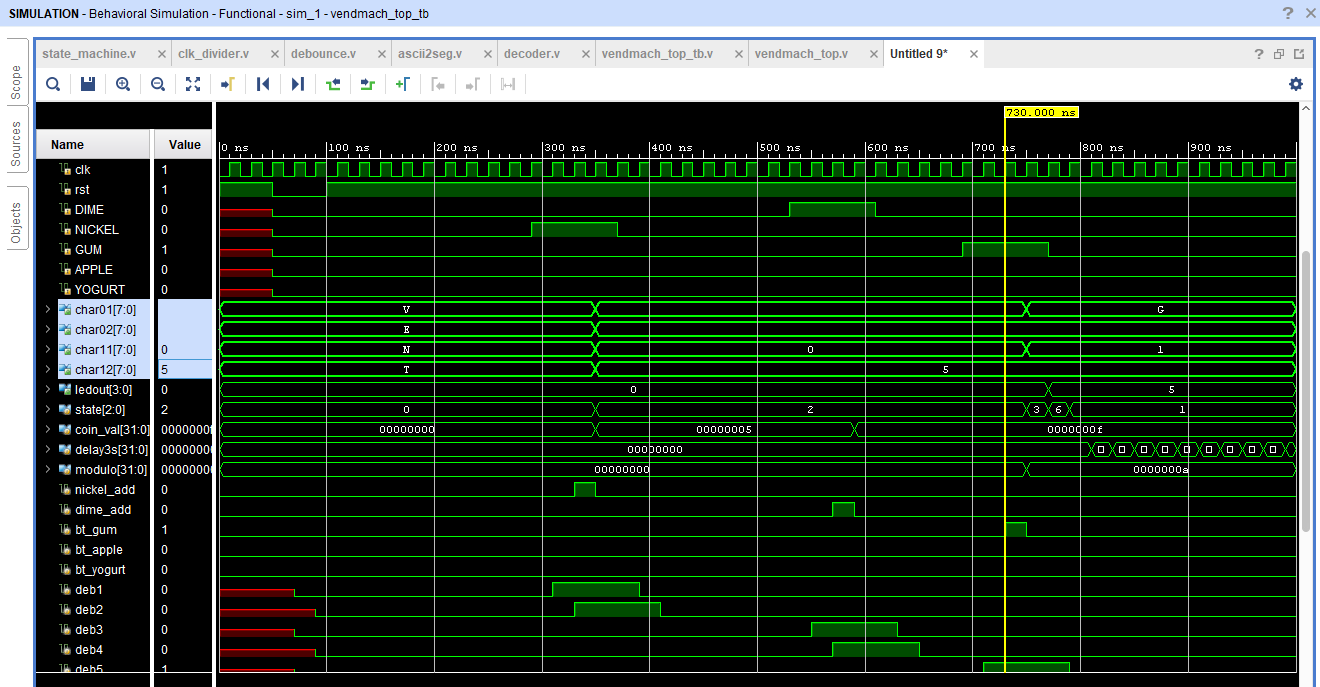
\includegraphics[width=1.0\textwidth ]{01_images/Simulation_state_machine.PNG}
	\caption{Vivado behavioral simulation of the state machine module.}
	\label{fig: Simulation_state_machine}
\end{figure}
%
%\subsection{Part I: behavioral simulation of decoder} \label{subsec: Part I: behavioral simulation of decoder}
%After a successful simulation of the synthesized hardware description language that implements an decoder a test bench was written, see listening \ref{lst: Testbanche decoder}. The time variant simulation is shown in figure \ref{fig: Vivado_lab1_BS} which shows steps trough the different possible switch positions and shows the output on the decoder bus seg. In comparison to the simulation given in Lab 02 Part 1 it could be confirmed that there are mostly identical.
%
%\begin{figure}[H]
%	\centering
%	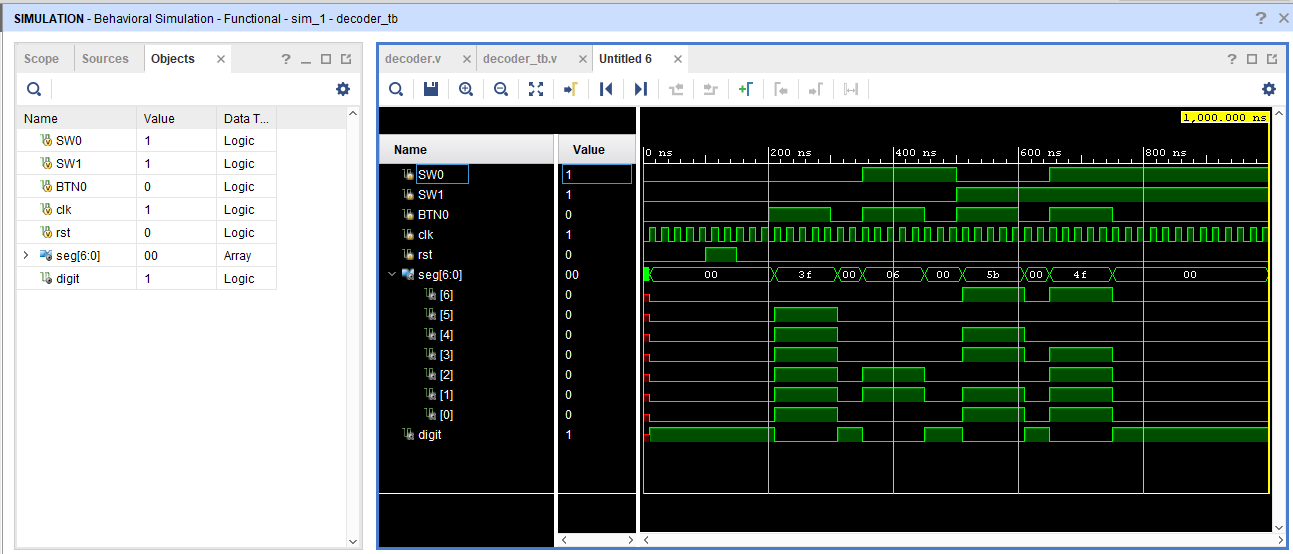
\includegraphics[width=1.0\textwidth ]{01_images/Vivado_lab2_BS.PNG}
%	\caption{Vivado behavioral simulation of the decoder module.}
%	\label{fig: Vivado_lab1_BS}
%\end{figure}
%
%\subsection{Part III: behavioral simulation of the Time Multiplexer} \label{Part III: behavioral simulation of the Time Multiplexer}
%The simulation was made to find bigs or logic faults in the code. Due to an extensive search of multiple hours to track down the issue stated in subsection \ref{subsubsec: Clock divider not working} which lead to the simulation shown in figure \ref{fig: Vivado_lab2_sim_time_multi_module}. The simulation shows how the simulation of an instantiated time multiplex module behaviors over time which indicates that the clock divider is working. Furthermore, It shows how the decoder witches the display to the first word and time multiplexes the displays with the switching carries line cat0 and cat1. 
%
%\begin{figure}[H]
%	\centering
%	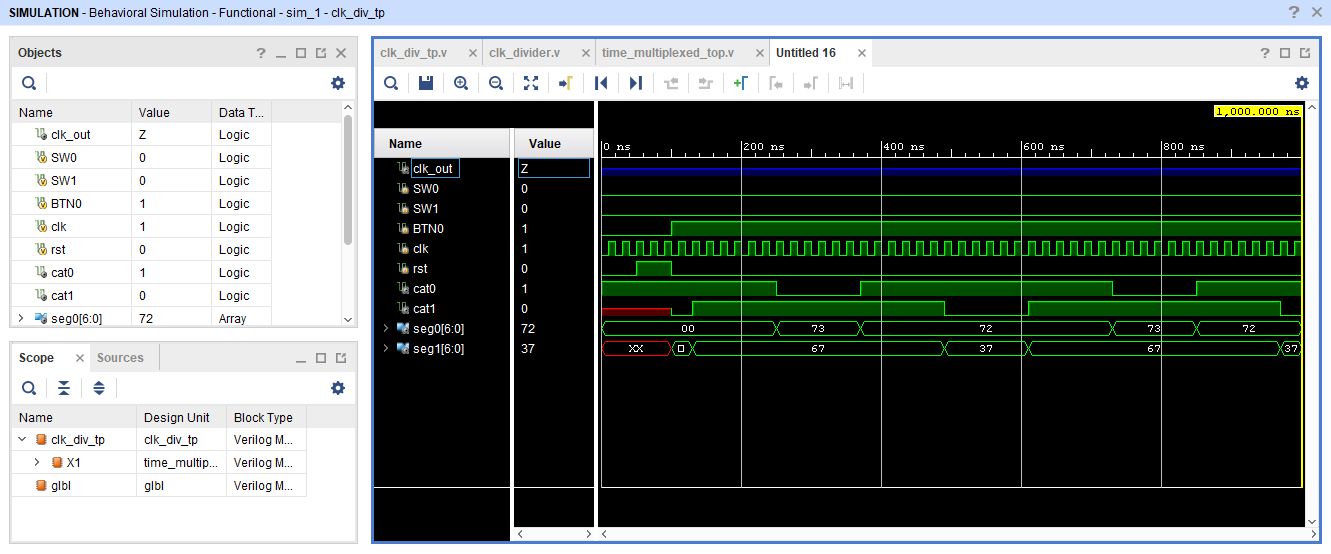
\includegraphics[width=1.0\textwidth ]{01_images/Vivado_lab2_sim_time_multi_module.PNG}
%	\caption{Vivado behavioral simulation of the decoder module.}
%	\label{fig: Vivado_lab2_sim_time_multi_module}
%\end{figure}
